%%%%%%%%%%%%%%%%%%%%%%%%%%%%%%%%%%%%%%%%%%%%%%%%%%%%%%%%%%%%%%%%%%%%%%%%%%%%%%%%%%%%%%%%%%%%%%%%%%%%%%%%%%%
%   \copyright 2013 Ricardo García Fernández - ricardogarfe [at] gmail [dot] com.
%
%    This work is licensed under a Creative Commons 3.0 Unported License.
%    To view a copy of this license visit:
% 
%    http://creativecommons.org/licenses/by/3.0/legalcode
%%%%%%%%%%%%%%%%%%%%%%%%%%%%%%%%%%%%%%%%%%%%%%%%%%%%%%%%%%%%%%%%%%%%%%%%%%%%%%%%%%%%%%%%%%%%%%%%%%%%%%%%%%

\chapter{Desarrollo de un proyecto}
\label{chap:desarrollo}

\par Cómo llevar a cabo el desarrollo de un proyecto con SCStack. Desarrollo en paralelo de un proyecto mediante github + travis-ci vs gerrit + jenkins.

\section{Alta usuarios}
\label{sec:alta-usuarios}

\par Dar de alta desarrolladores/Project Owners (usuarios de la forja).

% section alta-usuarios (end)

\section{Crear un proyecto}
\label{sec:crear-proyecto}

\subsection{Proyecto en redmine}
\label{sub:proyeto-redmine}

% subsection proyeto-redmine (end)

\subsection{Repositorio git}
\label{sub:repo-git}

\par Configurar usuario Git del desarrollador del proyecto para la forja:

\lstset{style=bashbasico}
\begin{lstlisting}[frame=trbl]
$ cat .gitconfig 
[user]
    name = patxigortazar
    email = patxi.gortazar@gmail.com
$ git config --global user.name "ricardogarfe"
$ git config --global user.email "ricardogarfe@gmail.com"
$ cd [path-to-gitrepo]
[path-to-gitrepo]$ git config user.name "ricardogarfe"
[path-to-gitrepo]$ git config user.email "ricardogarfe@gmail.com"
\end{lstlisting}

\par Comprobar las credenciales de Git en el ordenador del desarrollador:

\lstset{style=bashbasico}
\begin{lstlisting}[frame=trbl]$ git config --list
user.name=patxigortazar
user.email=patxi.gortazar@gmail.com
\end{lstlisting}

% subsection repo-git (end)

\subsection{Configuración de Jenkins}
\label{sub:jenkins-configuracion}

\par Configuracón de Jenkins para realizar determinadas tareas de forma automática:

\begin{itemize}
	\item Tags
	\item Construir las versiones vivas
\end{itemize}

\par También proveerá tareas para ser ejecutadas manualmente:

\begin{itemize}
	\item Branches de releases
	\item Desplegar una versión específica con un clic
\end{itemize}

\par Las versiones vivas vivirán en su propia máquina virtual

\begin{figure}[H]
    \centering
    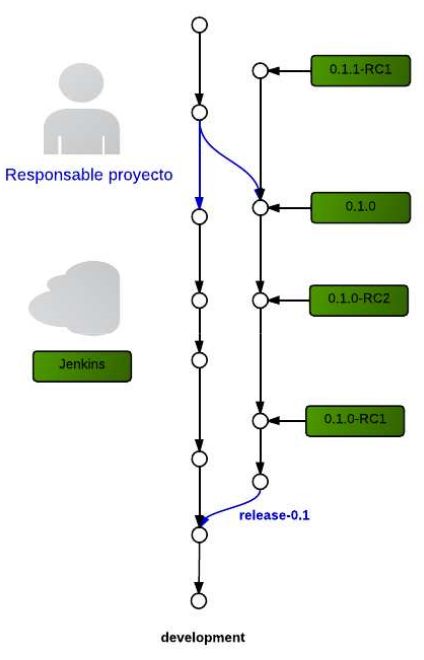
\includegraphics[width=0.6\textwidth]{jenkins-git}
    \caption{Jenkisn-Git relación en el proceso de integración}
    \label{fig:jenkins-git}
\end{figure}

\par Se mantendrán diferentes versiones vivas a la vez para cumplir unos objetivos con forme al desarrollo Iterativo e Incremental: \emph{'Release early, release often'}:

\begin{itemize}
	\item Asegurar la calidad
	\item Hacer el despliegue ágil
	\item Minimizar el riesgo
\end{itemize}

\par Para orientar la integración continua al proceso de desarrollo se ha de configurar \emph{Jenkins} para acceder a múltiples repositorios Git para esto se han de tener en cuenta los siguientes requerimientos:

\begin{itemize}
    \item \emph{Jenkins} construye diferentes proyectos en donde en proyecto puede tener su propio repositorio git.
    \item \emph{Jenkins} debe tener permisos de lectura o lectura/escritura a todos los repositorios de aquellos proyectos que vaya a construir.
    \item Por defecto \emph{Jenkins} usa la clave del usuario en \texttt{\ensuremath{\sim.ssh}} para autenticarse
    \item ¿Con qué usuario se ejecuta Jenkins? con el usuario \textbf{tomcat}.
\end{itemize}

\par El acceso de Jenkins a los distintos repositorios se configura a partir de un usuario por Jenkins repositorio, aislando los problemas descritos en la sección~\ref{sub:ci-jenkins} del capítulo \nameref{chap:procesos-desarrollo}.

\par Configurar \emph{Jenkins} para acceso a \emph{múltiples repositorios git} creando el usuario necesario en la Consola de Administración.

\begin{figure}[H]
    \centering
    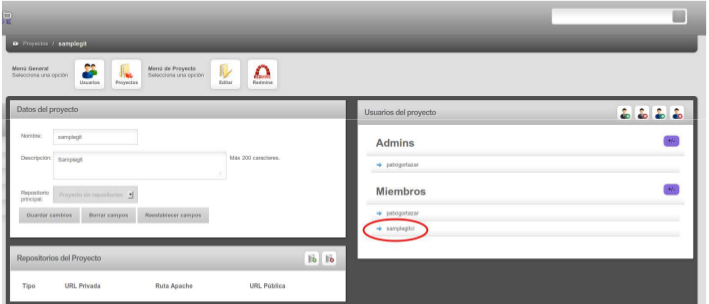
\includegraphics[width=\textwidth]{gestion-jenkins-usuarios-000}
    \caption{Crear usuarios para Jenkins a través de la consola de Administración}
    \label{fig:gestion-jenkins-usuarios-000}
\end{figure}

\par Generar un par de claves pública/privada con \texttt{ssh-keygen} para cada usuario en diferentes ficheros y acceder a Gerrit con cada usuario creado.

\begin{figure}[H]
    \centering
    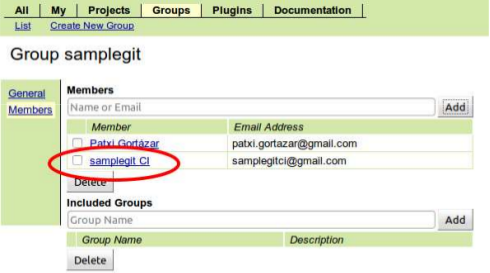
\includegraphics[width=\textwidth]{gestion-jenkins-usuarios-001}
    \caption{Configuración de usuarios Jenkisn en Gerrit}
    \label{fig:gestion-jenkins-usuarios-001}
\end{figure}

\par Añadir la clave pública para este usuario para copiar las claves al servidor de Jenkins en el directorio\texttt{'/opt/ssh-keys'}.

\lstset{style=bashbasico}
\begin{lstlisting}[frame=trbl]
$ git config --list
$ cd /opt/ssh-keys
$ ll
total 24
drwxr-xr-x  2 tomcat tomcat 4096 Jan  4 09:46 ./
drwxr-xr-x 14 root   root   4096 Jan  4 09:42 ../
- rw-------  1 tomcat tomcat 1679 Jan  4 09:46 filetransferci_rsa
- rw-r--r--  1 tomcat tomcat  398 Jan  4 09:46 filetransferci_rsa.pub
- rw-------  1 tomcat tomcat 1679 Jan  4 09:44 samplegitci_rsa
- rw-r--r--  1 tomcat tomcat  396 Jan  4 09:44 samplegitci_rsa.pub
</code>
\end{lstlisting}

\par Configurar SSH para que utilice la clave correcta en cada caso creando el fichero \texttt{/home/tomcat/.ssh/config}.

\lstset{style=bashbasico}
\begin{lstlisting}[frame=trbl]
$ git config --list
$ cd /home/tomcat/.ssh
$ cat config
Host samplegit.ricardogarfe.sidelab.es
    HostName ricardogarfe.sidelab.es
    User samplegitci
    IdentityFile /opt/ssh-keys/samplegitci_rsa
Host filetransfer.ricardogarfe.sidelab.es
    HostName ricardogarfe.sidelab.es
    User filetransferci
    IdentityFile /opt/ssh-keys/filetransferci_rsa
\end{lstlisting}

\subsection{Configuración de builds}
\label{sub:jenkins-build-jobs}

\par Los builds de \emph{Jenkins} funcionan a través de la configuración de \textbf{jobs}. Por lo que vamos a definir los jobs necesarios para el proceso de integración continua. Se dividen en tres grupos:

\begin{itemize}
    \item Jobs de \textbf{integración} (read only).
        \begin{itemize}
            \item Descargan el código (checkout).
            \item Construyen.
            \item Pasan tests.
            \item Despliegan la versión construida en ``local''.
        \end{itemize}
    \item Jobs de \textbf{release} (read/write).
        \begin{itemize}
            \item Realizan los pasos anteriores y además.
            \item Tag si los tests pasaron.
            \item Push del tag al repositorio remoto.
        \end{itemize}
    \item Jobs de \textbf{despliegue} (read only).
        \begin{itemize}
            \item Descargan el binario del repositorio de binarios
            \item Desplegar
        \end{itemize}
\end{itemize}

\subsubsection{Job de integración}
\label{subs:jenkins-job-integracion}

\par Configurar el job de integración mediante Maven:

\begin{itemize}
	\item Crear un \textbf{job} \emph{Maven}.
	\item Configurar el repositorio git:
        \begin{itemize}
	        \item \emph{ssh://filetransferci@filetransferci.code.tscompany.es/filetransfer}
	        \item Ssh leerá el fichero config y utilizará el fichero de claves correspondiente el host \texttt{filetransferci.code.tscompany.es}.
        \end{itemize}
	\item Añadir las ramas a construir (añadir nuevas ramas con el botón ``Add'')
        \begin{itemize}
	        \item development
	        \item release-0.1.1
        \end{itemize}
	\item Añadir el \texttt{user.email} y \texttt{user.name} que usará \emph{Jenkins}.
        \begin{figure}[H]
            \centering
            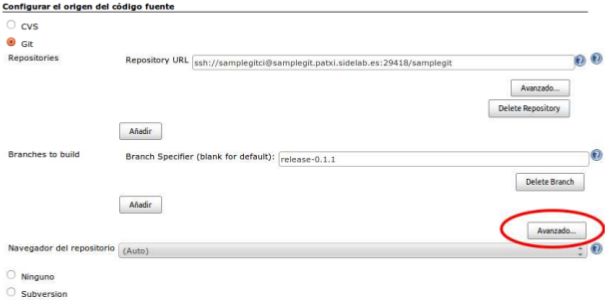
\includegraphics[width=0.7\textwidth]{jenkins-job-integracion}
            \caption{Crear Job integración en Jenkins}
            \label{fg:jenkins-job-integracion}
        \end{figure}
	\item Los resultados del build se pueden comprobar en: 
        \begin{itemize}
	        \item \texttt{/opt/jenkins/jobs/filetransfer/workspace}
	        \item Si es un proyecto \emph{Maven}, dentro del proyecto en la carpeta target estará el artefacto generado.
	        \item También se puede acceder vía web y descargar el workspace como un zip.
	        \item Los \textbf{tests} están en la carpeta \texttt{surfire-reports} del proyecto \emph{Maven}.
	        \item También pueden consultarse vía web accediendo al build y seleccionando \emph{'Resultado de los tests'}.
        \begin{figure}[H]
            \centering
            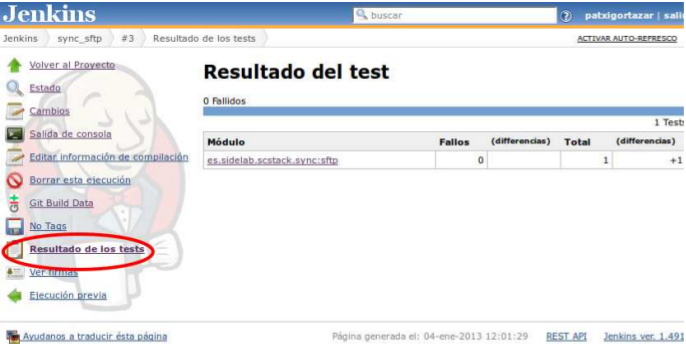
\includegraphics[width=\textwidth]{jenkins-job-resultados}
            \caption{Resultados de los test a través de la interfaz de Jenkins}
            \label{fig:jenkins-job-resultados}
        \end{figure}
        \end{itemize}
\end{itemize}

\subsection{Maven}
\label{sub:jenkins-maven}

\par \emph{Jenkins} permite construir proyectos \emph{Maven}.

\par En determinadas ocasiones los proyectos requieren configuraciones específicas. La información sensible suele ir en el fichero \texttt{settings.xml} en el \texttt{home} del usuario en su máquina de desarrollo.

\begin{itemize}
    \item Info de \textbf{autenticación para Archiva}.
    \item \textbf{Profiles}
\end{itemize}

\par En Jenkins esto se puede gestionar con el plugin \emph{``Config File Provider Plugin''}.

\begin{figure}[H]
    \centering
    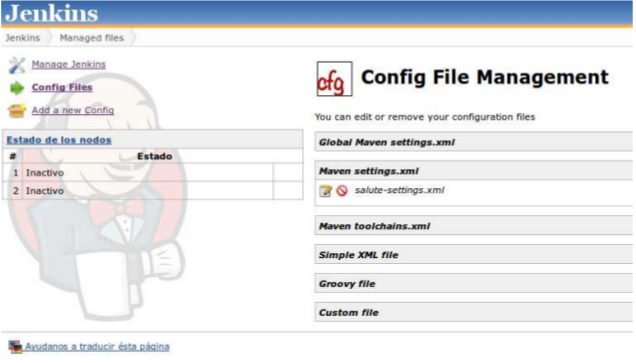
\includegraphics[width=\textwidth]{jenkins-config-file-management}
    \caption{Configuración de Maven a través de Jenkins}
    \label{fig:jenkins-config-file-management}
\end{figure}

\par Podemos añadir cualquiera de los ficheros creados con \emph{Config File Management} en un \textbf{job}.

\begin{figure}[H]
    \centering
    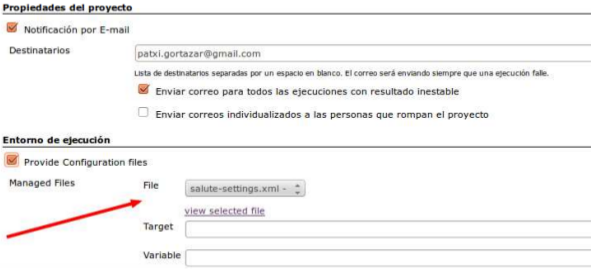
\includegraphics[width=\textwidth]{jenkins-config-file-management-settings}
    \caption{Seleccionar archivo de configuración de Maven}
    \label{fig:jenkins-config-file-management-settings}
\end{figure}

\par Para los deploys, si el certificado es autofirmado es \textbf{necesario} generar un \textbf{truststore} a partir del certificado generado por el servidor\footnote{\url{http://www.liferay.com/web/neil.griffin/blog/-/blogs/fixing-suncertpathbuilderexception-caused-by-maven-downloading-from-self-signed-repository}}.

\par Este truststore debe incluirse en todos los \texttt{jdk} que utilice \emph{Jenkins} en la ruta indicada en el enlace anterior.

% subsection jobs-jenkins (end)

% section crear-proyecto (end)

\section{Proceso de desarrollo basado en ramas}
\label{sec:desarrollo-en-ramas}

\par Proceso de desarrollo basado en ramas partiendo de 2 ramas de forma continua:

\begin{itemize}
    \item \textbf{master:} Desarrollo limpio. Sólo versiones estables.
    \item \textbf{develop:} El desarrollo inicial de la versión actual tiene lugar aquí.
\end{itemize}

\par Gestión de las ramas para estabilización de las versiones:

\begin{itemize}
    \item \textbf{release-0.1}, \textbf{release-0.2}; una rama de estabilización cada vez   
\end{itemize}

\subsection{Proceso de estabilización}

\par El proceso de estabilización se gestiona a través de las \emph{ramas de estabilización}:

\begin{itemize}
    \item Estabilización del código (\emph{RC release candidates})
    \item Arreglar bugs (hotfixes)
    \item Cuando la versión se considera estable se procede al siguiente paso:
        \begin{itemize}
            \item Tag
            \item Mezclar (merge) con development
            \item Mezclar (merge) con master
        \end{itemize}
    \item Si surgen nuevos bugs se vuelve a repetir el \textbf{proceso de estabilización}:
        \begin{itemize}
            \item Se arreglan en la misma rama (release-0.1)
            \item Nuevo tag y mezcla
        \end{itemize}
\end{itemize}

\subsection{Releasing}

\par Para crear una Release se define un proceso de gestión a través las ramas:

\begin{itemize}
    \item Checkout del tag
    \item Build (Jenkins)
    \item Deploy (Jenkins)
\end{itemize}

\subsection{Diagrama de desarrollo}

\par El flujo de trabajo a través de las ramas se representa en este diagrama:

\begin{figure}[H]
\centering
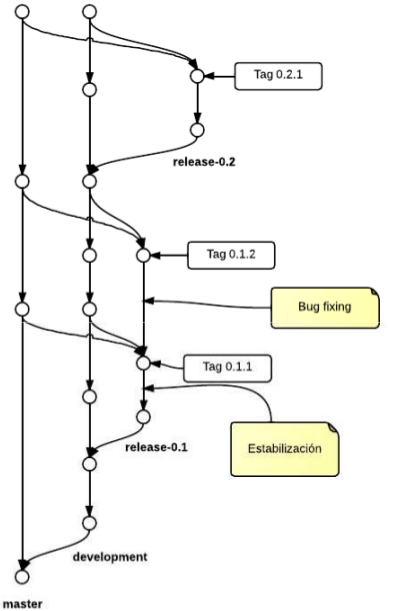
\includegraphics[width=0.6\textwidth]{flujo-desarrollo-git-000}
\caption{Flujo de desarrollo Git.}
\label{fig:flujo-desarrollo-git-000}
\end{figure}

% section desarrollo-en-ramas (end)

%%%%%%%%%%%%%%%%%%%%%%%%%%%%%%%%%%%%%%